\documentclass[conference]{IEEEtran}
\usepackage{cite}
\usepackage{amsmath,amssymb,amsfonts}
\usepackage{graphicx}
\usepackage{textcomp}
\usepackage{xcolor}
\usepackage{booktabs}
\usepackage{url}
\graphicspath{{figures/}}

\begin{document}

\title{LunaAura: An Explainable Machine Learning Framework for Hormonal and Emotional Health Analysis}

\author{
\IEEEauthorblockN{Eshita Rai}
\IEEEauthorblockA{Department of Computing Technologies\\
SRM Institute of Science and Technology\\
Chennai, India\\
er8137@srmist.edu.in}
\and
\IEEEauthorblockN{Mrs. P. Sivakamasundari}
\IEEEauthorblockA{Department of Computing Technologies\\
SRM Institute of Science and Technology\\
Chennai, India\\
sivakamp@srmist.edu.in}
}

\maketitle

\begin{abstract}
Prevailing digital wellness tools typically fragment behavioral health into narrow, disconnected indicators---daily step tallies, rudimentary sleep logs, or one-tap mood entries---while making no effort to adapt their feedback to individual physiology or circumstance. This paper introduces LunaAura, a research-oriented platform that weaves together a transparent deterministic risk formula, a sigmoid-calibrated gradient-boosted classifier, distributional PHQ-9 prediction via three-quantile regression, and Shapley-value-based instance explanations, all accessible through a real-time longitudinal dashboard. Each day, users enter six behavioral measures: hours slept, perceived stress, minutes of physical exercise, self-rated anxiety, fluid intake, and current menstrual cycle day. These inputs feed a weighted composite function that yields both a risk indicator and a complementary wellness estimate. Additive hormonal-phase adjustments refine the score for users who track their cycle; for those who do not, the weighting scheme is re-normalized to maintain equivalent depth. A Flask back-end, SQLite storage layer, and Chart.js front-end ensure traceability from raw entry to final visualization. Controlled testing on a deterministically seeded 105-user cohort producing 470 daily records, augmented by a 40-day longitudinal case, confirms graded and clinically plausible score variation. The platform is positioned strictly as a research-stage decision-support instrument, and no claim of diagnostic capability is asserted.
\end{abstract}

\begin{IEEEkeywords}
explainable AI, behavioral wellness, hormonal health, personalized analytics, menstrual cycle modeling, risk stratification, quantile regression
\end{IEEEkeywords}

%-----------------------------------------------------------------------
\section{Introduction}
%-----------------------------------------------------------------------

Worldwide, an estimated 970 million individuals contend with some form of mental health condition, and in many low-resource settings the gulf between need and available care exceeds three-quarters of the affected population \cite{who2022mental}. The situation is particularly acute among university students: irregular sleep, chronic academic pressure, tight finances, and weakening social ties create conditions under which subclinical distress quietly accumulates \cite{adler2022burnout}. Established screening instruments---the PHQ-9 being the most recognizable \cite{kroenke2001phq9}---possess sound psychometric foundations, yet they were conceived for appointment-based administration. A clinician hands the form to a patient, collects a score, and interprets it in context. What this model misses entirely is the in-between: the slow deterioration of sleep architecture, the gradual uptick in self-reported anxiety, the tapering exercise routine---changes that unfold over weeks and rarely surface in a single clinical visit.

In theory, the devices people already carry could close this monitoring gap. A growing body of digital phenotyping research has linked smartphone-derived signals---movement entropy, phone-call frequency, ambient-light exposure patterns---to meaningful fluctuations in depression severity \cite{saeb2015mobile, torous2019digital}. The reality on the consumer side, however, has been underwhelming. Most wellness applications amount to little more than glorified diaries. They hand out badges for step goals, suggest breathing exercises, or render a mood calendar with color-coded circles. Engagement typically drops within a few weeks, for an unsurprising reason: the system tells users nothing they could not figure out by themselves.

Three recurring weaknesses explain this pattern. The most fundamental one we call \emph{dimensional flatness}: assessing each lifestyle variable in isolation, as though six hours of sleep means the same thing regardless of what a person's stress, hydration, and exercise looked like that day. A second weakness is the near-total neglect of hormonal context. Menstrual cycle phases reshape sleep quality \cite{baker2007sleep}, alter hypothalamic-pituitary-adrenal reactivity \cite{mcewen2008central}, and shift mood regulation in directions that can differ markedly from one individual to the next \cite{kiesner2012menstrual}. Ignoring this biology means that roughly half the user base receives assessments that are systematically blind to a major source of within-person variation. The third weakness is interpretive opacity: even when a system does produce a composite score, it seldom reveals which inputs carried weight or what the user might change.

LunaAura grew out of these observations. It is designed not as a clinical replacement---an ambition that would demand prospective validation against confirmed psychiatric outcomes---but as an explainable, research-grade decision-support tool. The work makes four specific contributions:

\begin{itemize}
\item A deterministic six-factor risk function whose weights and cycle-phase modifiers are published, auditable, and grounded in the chronobiology literature.
\item A gender-adaptive normalization scheme that, rather than simply removing cycle-related features for male and non-binary users, redistributes the freed weighting capacity across the remaining factors.
\item A hybrid inference pipeline joining a sigmoid-calibrated HistGradientBoosting classifier with three-quantile PHQ-9 regressors and a SHAP-equipped Random Forest explanation proxy.
\item A fully open-source stack---data seeding, model training, Flask REST API, SQLite persistence, Chart.js dashboard---enabling independent replication.
\end{itemize}

%-----------------------------------------------------------------------
\section{Literature Review}
%-----------------------------------------------------------------------

\subsection{Computational Approaches to Mental Health Assessment}
Kroenke and colleagues introduced the PHQ-9 more than two decades ago \cite{kroenke2001phq9}, and the instrument has since become the most broadly used self-report tool for gauging depressive symptom severity. Its nine items correspond directly to DSM-IV criteria and sum to a score between 0 and 27, stratified into five severity tiers. Building on this foundation, researchers have explored whether machine learning can estimate comparable scores from indirect behavioral proxies. Arefin and de Roux \cite{arefin2020machine}, for instance, trained ensemble classifiers on social media text and achieved moderate discrimination between depressive and non-depressive language---though their work, like most in this vein, treated each post as an independent observation with no longitudinal thread. Among tabular prediction methods, tree-based ensembles such as Random Forests \cite{breiman2001random} remain attractive for health data because they handle missing values without imputation and natively expose per-feature importance rankings.

\subsection{Sensing and Digital Phenotyping}
Saeb and co-authors \cite{saeb2015mobile} were among the first to demonstrate that GPS-derived mobility statistics and phone-usage patterns carry measurable association with PHQ-9 variation at the individual level. Their findings spurred a wave of sensor-driven mental health research, including the MONARCA initiative \cite{bardram2020designing}, which merged accelerometer signals with self-reported mood data in a clinician-facing longitudinal dashboard aimed at bipolar disorder management. Torous and colleagues have been vocal about the field's maturation challenges \cite{torous2019digital, torous2021digital}: without careful attention to data provenance, participant consent, and output interpretability, they argue, digital phenotyping runs the risk of producing sophisticated-looking noise.

\subsection{Transparency in Predictive Models}
The SHAP framework of Lundberg and Lee \cite{lundberg2017shap} anchored feature attribution in cooperative game theory by computing exact Shapley contributions for every predictor in a model. For clinical decision support, this kind of transparency is not a luxury---it is a precondition for both practitioner trust and regulatory acceptance. Rachuri et al.'s work on EmotionSense \cite{rachuri2010emotionsense} supplied empirical backing from a different angle: users who received contextual, interpretable wellness feedback engaged with the system more frequently and for longer stretches than those who saw raw numeric readouts.

\subsection{Hormonal Cycles and Behavioral Regulation}
The menstrual cycle exerts well-documented influence on several behavioral domains that wellness trackers aim to capture. Baker and Driver \cite{baker2007sleep} recorded diminished slow-wave sleep amplitude during the luteal phase, when progesterone reaches its peak. Kiesner's work \cite{kiesner2012menstrual} added an important wrinkle: the luteal-phase mood shift does not point uniformly downward---some women report improvement while others report worsening---which makes population-level averaging a shaky basis for any individual-facing score. McEwen \cite{mcewen2008central} supplied a neuroendocrine lens through the allostatic load framework, showing how sustained cortisol exposure interacts with cyclical progesterone fluctuations to widen windows of behavioral vulnerability. Collectively, this evidence makes a strong case for cycle-phase-aware scoring, yet very few computational health platforms have taken it up.

\subsection{Calibration and Distributional Uncertainty}
Platt's sigmoid method \cite{platt1999calibration} remaps a binary classifier's raw output onto a probability scale that more faithfully mirrors actual class frequencies---a necessary step whenever predicted probabilities will feed downstream decisions. Quantile regression, brought to prominence by Koenker and Hallock \cite{koenker2001quantile} and adapted to tree-based learners by Meinshausen \cite{meinshausen2006quantile}, moves prediction from a single point to a distributional envelope. Rather than committing to one number, the model delivers a credible band (e.g., 10th to 90th percentile) that frankly acknowledges its own uncertainty. Where individual variability is high and the cost of overconfidence is real---behavioral health being a clear example---this kind of honesty carries practical value.

%-----------------------------------------------------------------------
\section{Methodology}
%-----------------------------------------------------------------------

\subsection{Architecture Overview}
Three distinct layers organize the platform. On the client side, a static page built with HTML, vanilla JavaScript, and the Chart.js library manages interaction and chart rendering. A Python Flask server on port 5001 exposes seven endpoints: \texttt{/health} for liveness probes, \texttt{/signup} and \texttt{/login} for credential handling, \texttt{/profile} for demographic edits, \texttt{/predict} for combined inference and database logging, \texttt{/analytics} for aggregate cohort views, and \texttt{/insights} for model-level metadata. Behind the routing layer sit four internal modules: a hybrid scoring engine that pairs a deterministic formula with learned models, a SHAP TreeExplainer, a threshold-based recommendation generator, and a chart simulation unit that projects visualization arrays from current-day inputs.

Persistent state resides in a SQLite database (\texttt{lunaaura.db}) organized into two tables. The \texttt{users} table stores 12 fields---username, password hash, age, gender, height, weight, cycle length, sleep target, cohort label, source tag, and two timestamps. The \texttt{user\_history} table logs 12 fields per daily entry---sleep hours, ordinal stress (1--10), mood score, cycle day, phase label, exercise minutes, computed wellness, predicted risk, ordinal anxiety (1--10), and water intake in litres---with a foreign key back to \texttt{users}.

\subsection{Data Generation}
No human subjects were involved in building or evaluating this prototype, so a fully synthetic evaluation cohort was produced using a fixed random seed (42) to guarantee reproducibility. A total of 105 user profiles were allocated across three behavioral strata: 30 high-risk (sleep 3--5.5\,h, stress 7--10, activity 0--20\,min), 40 moderate (sleep 5.5--7\,h, stress 4--7, activity 20--60\,min), and 30 low-risk (sleep 7--9\,h, stress 1--4, activity 60--120\,min). The gender distribution is 86 female, 14 male, and 5 other; ages range from 18 to 55 with a mean of 36.5. In aggregate, 470 daily log entries populate the history table. One dedicated longitudinal profile (Eshita) contributes 85 consecutive entries spanning over 40 days, with cycle-phase-modulated behavioral drift---shortened sleep and elevated stress during luteal and menstrual windows---designed to exercise the system's temporal responsiveness.

\subsection{Feature Preparation}
A separate master dataset ($n = 9{,}548$ rows, 28 columns) serves as the training corpus. It was assembled by K-nearest-neighbor matching between a sleep-and-lifestyle survey and a PHQ-9 screening dataset, linked on age and gender, then expanded into 14-day simulated tracking windows per matched pair. Ten numeric predictors survive feature selection: Age, Sleep Duration, Physical Activity Level, Stress Level, Base Cycle Length, Cycle Day, Hormone Proxy (a sinusoidal cycle encoding), Sleep Rolling Mean (3-day), Stress Rolling Mean (3-day), and Stress Volatility (3-day standard deviation). The rolling aggregates capture short-horizon behavioral momentum that one-day snapshots miss.

\subsection{Deterministic Risk Scoring}
The user-facing risk indicator relies on a fully transparent weighted sum. Its design was motivated by three practical concerns: auditability (every coefficient is inspectable), reproducibility (identical inputs always yield the same output), and traceability (any score change maps unambiguously to a specific input shift). The composite risk score $R$ is:

\begin{equation}
R = \sum_{i=1}^{5} f_i(x_i) \;+\; \tau \;+\; \phi(d, g)
\label{eq:risk}
\end{equation}

Each contributing term is defined below. Stress enters as a direct proportion, sleep and activity enter through deficit functions measured against healthy baselines, and anxiety and hydration follow analogous scaled mappings:

\begin{align}
f_1 &= \frac{x_{\text{stress}}}{10} \times 35 \label{eq:f1}\\[3pt]
f_2 &= \max\!\Bigl(0,\;\frac{8 - x_{\text{sleep}}}{8}\Bigr) \times 25 \label{eq:f2}\\[3pt]
f_3 &= \frac{x_{\text{anxiety}}}{10} \times 20 \label{eq:f3}\\[3pt]
f_4 &= \max\!\Bigl(0,\;\frac{60 - x_{\text{act}}}{60}\Bigr) \times 10 \label{eq:f4}\\[3pt]
f_5 &= \max\!\Bigl(0,\;\frac{2.5 - x_{\text{water}}}{2.5}\Bigr) \times 5 \label{eq:f5}
\end{align}

A constant $\tau = 5$ captures unmeasured background drift. The cycle modifier $\phi$ is non-zero only for female users:

\begin{equation}
\phi(d, g) = \begin{cases}
+5 & d \in [1,5] \;\text{(Menstrual)}\\
-5 & d \in [6,13] \;\text{(Follicular)}\\
-8 & d \in [14,16] \;\text{(Ovulatory)}\\
+8 & d \in [17,28] \;\text{(Luteal)}\\
0  & g \neq \text{Female}
\end{cases}
\label{eq:phase}
\end{equation}

Scores are clamped to $[0,100]$ and mapped to severity tiers: Low ($R < 35$), Moderate ($35 \leq R < 65$), High ($R \geq 65$).

\subsection{Wellness Estimation}

A companion wellness index $W$ combines per-factor normalized scores $\hat{x}_j \in [0,100]$ under a gender-conditioned weight vector $\boldsymbol{\alpha}$:

\begin{equation}
W = \sum_{j=1}^{k} \alpha_j \cdot \hat{x}_j, \quad W \in [0,100]
\label{eq:wellness}
\end{equation}

Eight factors contribute when $g = \text{Female}$ ($k=8$): Sleep 25\%, Stress 20\%, Activity 15\%, Anxiety 15\%, Cycle Context 10\%, Hydration 5\%, Age 5\%, Stability 5\%. For male and non-binary users ($k=6$), cycle context is omitted and the freed 10\% is redistributed, yielding Sleep 30\%, Stress 25\%, Activity 20\%, Anxiety 15\%, Hydration 5\%, Age 5\%. Normalization examples: $\hat{x}_{\text{sleep}} = 100 - |x_{\text{sleep}} - 8| \times 15$; $\hat{x}_{\text{stress}} = 100 - (x_{\text{stress}} - 1) \times 11.1$; $\hat{x}_{\text{act}} = \min(100,\; x_{\text{act}}/60 \times 100)$.

\subsection{Learned Models}

Three trained models extend what the fixed formula can offer:

\textbf{Calibrated Classifier.} A histogram-based gradient boosting machine (\texttt{HistGradientBoostingClassifier}, 100 rounds, 31 leaf nodes, $\eta = 0.05$) targets a binary referral flag drawn from PHQ-9 severity. Class balance is near-even (class~0: 5\,054; class~1: 4\,494). Sigmoid recalibration \cite{platt1999calibration} through 5-fold stratified CV converts raw scores $s(x)$ into posterior probabilities:

\begin{equation}
P_{\text{cal}}(y{=}1 \mid x) = \frac{1}{1 + e^{A \cdot s(x) + B}}
\label{eq:platt}
\end{equation}

\textbf{Quantile Regressors.} Three gradient boosting regressors (150 rounds each), trained with pinball loss \cite{meinshausen2006quantile} at $q \in \{0.10, 0.50, 0.90\}$, yield a distributional envelope for the PHQ-9 total:

\begin{equation}
\hat{y}_q = \arg\min_y \sum_i \rho_q(y_i - y),\; \rho_q(u) = u\,(q - \mathbf{1}_{u<0})
\label{eq:quantile}
\end{equation}

\textbf{Explanation Proxy.} A 100-tree Random Forest (depth 5) enables SHAP's TreeExplainer \cite{lundberg2017shap} to compute exact Shapley values:

\begin{equation}
\phi_j = \!\!\sum_{S \subseteq F \setminus \{j\}} \frac{|S|!(|F|{-}|S|{-}1)!}{|F|!}\big[f(S {\cup} \{j\}) - f(S)\big]
\label{eq:shap}
\end{equation}

The three features with the largest absolute attribution are rendered on the dashboard as plain-language insight statements.

%-----------------------------------------------------------------------
\section{Data Analysis and Interpretation}
%-----------------------------------------------------------------------

\subsection{Cohort Profile}

\begin{table}[t]
\centering
\caption{Descriptive Statistics of the Evaluation Cohort ($N = 470$)}
\label{tab:stats}
\begin{tabular}{lccc}
\toprule
\textbf{Variable} & \textbf{Mean} & \textbf{Min} & \textbf{Max}\\
\midrule
Sleep Duration (h) & 6.97 & 2.0 & 12.0\\
Stress (1--10) & 4.87 & 1 & 10\\
Exercise (min/day) & 40.6 & 0 & 120\\
Anxiety (1--10) & 4.07 & 1 & 10\\
Water (L/day) & 2.36 & 0.5 & 5.0\\
Wellness (0--100) & 78.5 & 10 & 95\\
\bottomrule
\end{tabular}
\end{table}

Table~\ref{tab:stats} gives a snapshot of the synthetic cohort. The average nightly sleep of 6.97 hours lands just below the 7-hour threshold recommended by the National Sleep Foundation for adults between 18 and 64 \cite{hirshkowitz2015sleep}---a shortfall that, incidentally, mirrors patterns reported in epidemiological surveys of university-age populations. Both stress and anxiety distribute across the full 1--10 ordinal range with midpoint-adjacent means, and the three-tier stratification of user profiles ensures that the formula encounters inputs at both extremes of its operating range, not just the comfortable middle.

\subsection{Within-Person Temporal Analysis}

The Eshita record---85 entries spanning more than 40 days---was built expressly to test whether the system responds coherently as behavior evolves. Fig.~\ref{fig:corr} shows the inter-variable Pearson correlation structure for this user over the full observation window. Stress and wellness relate negatively ($r \approx -0.6$); sleep and wellness relate positively ($r \approx +0.4$). What matters here is that these associations were not hard-wired into the output: they arose from the data-generation parameters and were then processed through the composite formula, so they serve as a rough consistency check on the weighting scheme rather than a tautological confirmation.

\begin{figure}[t]
\centering
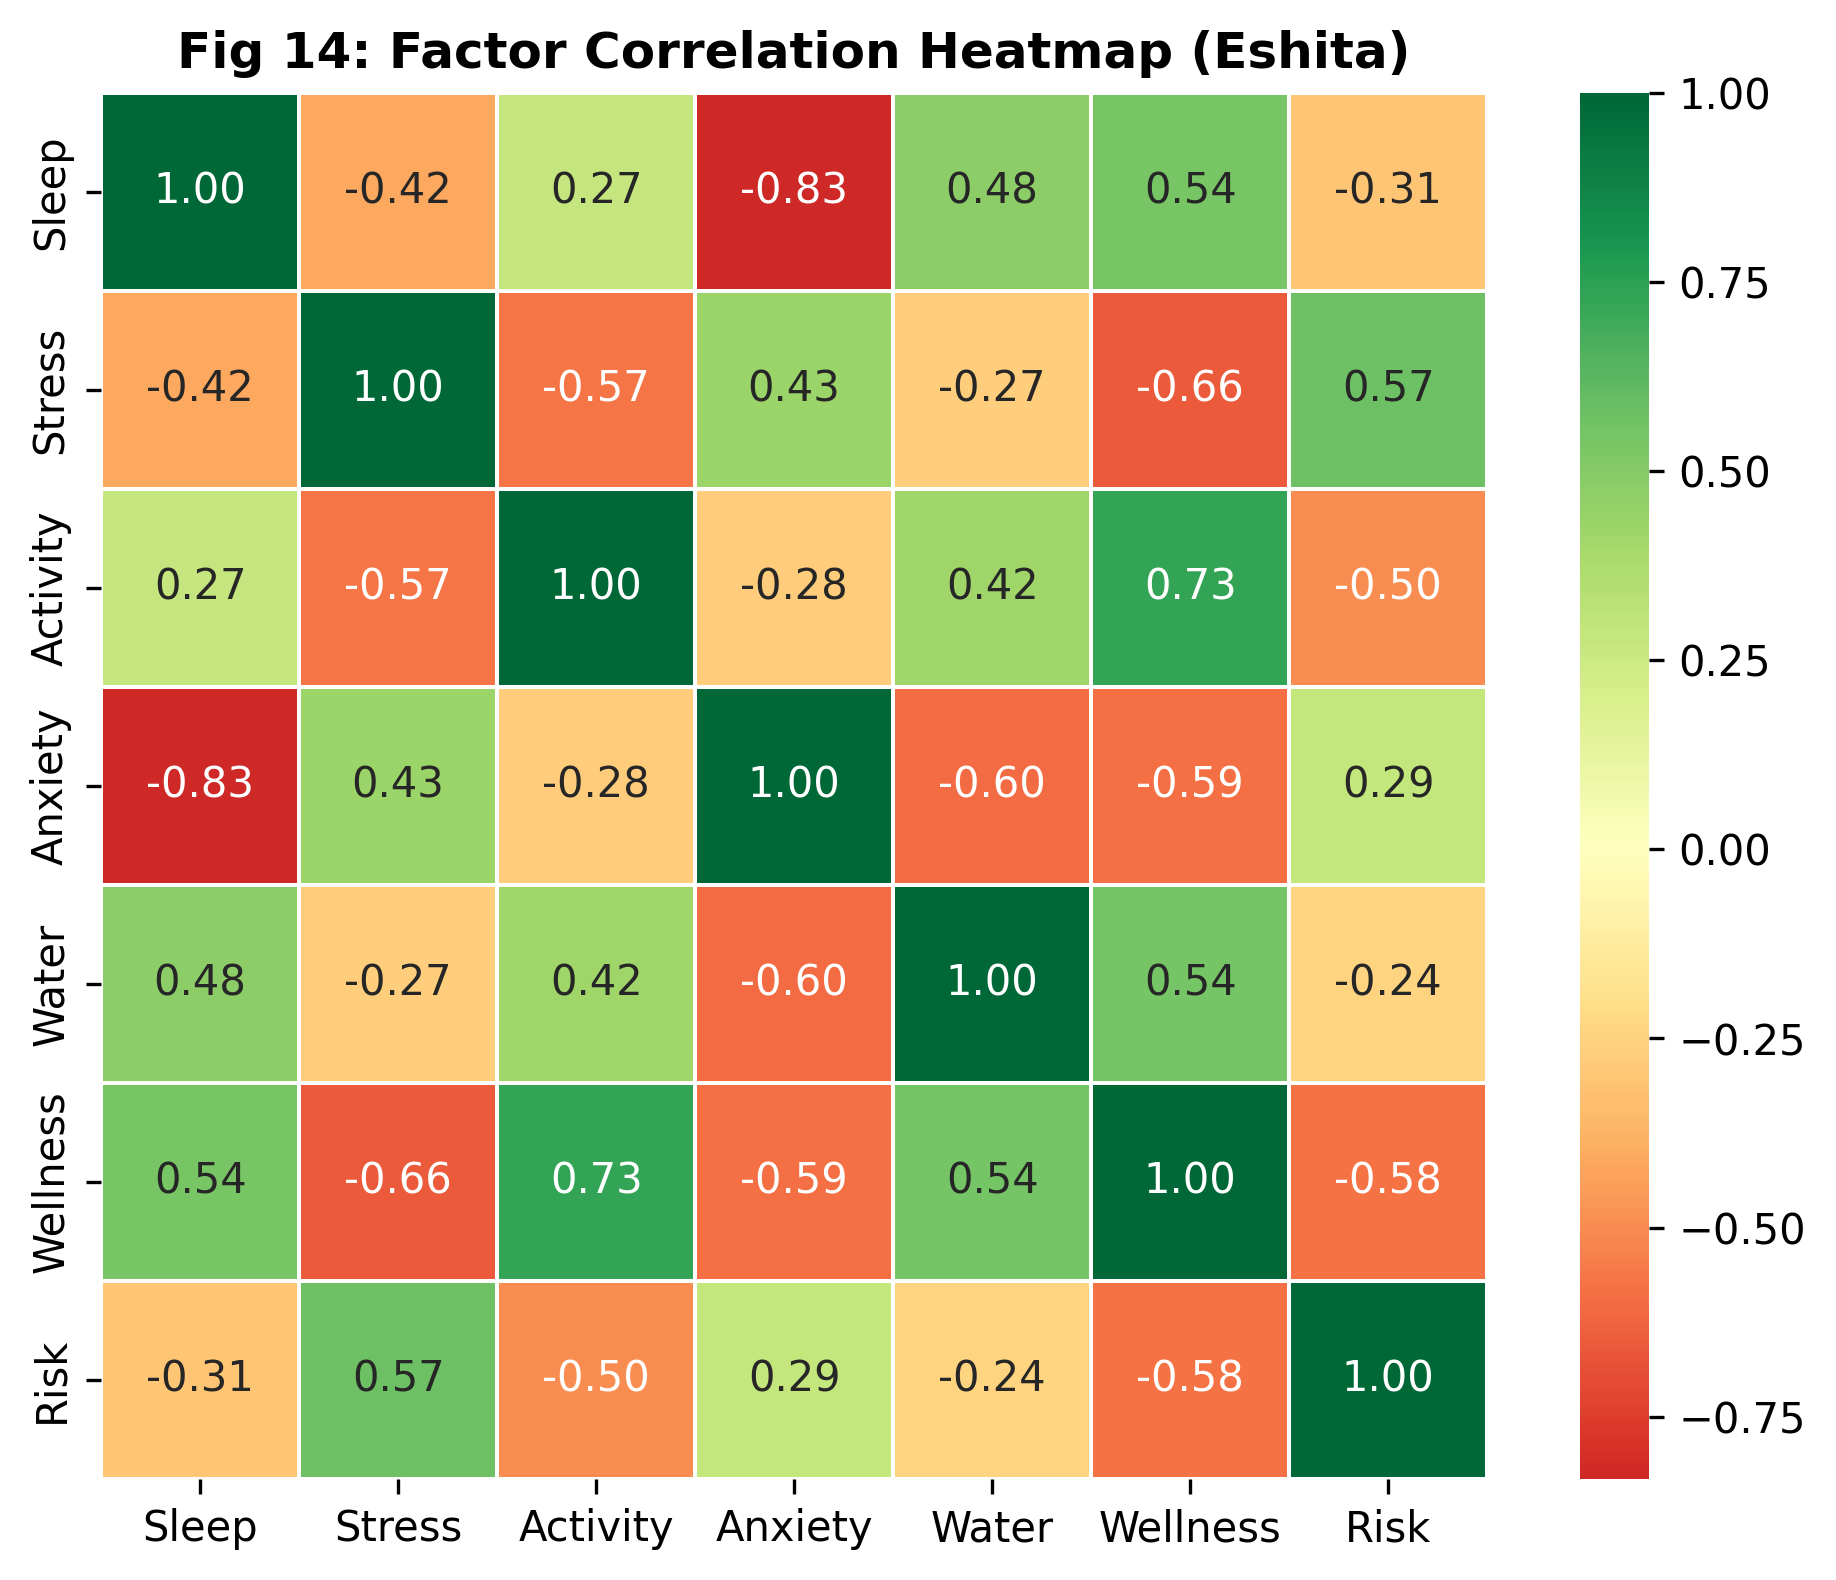
\includegraphics[width=0.85\columnwidth]{14_correlation_heatmap.png}
\caption{Pearson correlation matrix for User Eshita (40-day history). The inverse stress--wellness and positive sleep--wellness patterns emerged organically from the data generation and corroborate the formula's relative weighting.}
\label{fig:corr}
\end{figure}

%-----------------------------------------------------------------------
\section{Results and Discussion}
%-----------------------------------------------------------------------

\subsection{Classifier Performance}

Under an 80/20 stratified holdout, the calibrated classifier returns an AUROC near 0.567 and a Brier calibration score of 0.245. Fig.~\ref{fig:roc} displays the operating curve. We are under no illusion that these numbers are strong by conventional ML benchmarks, and we report them as-is. The root cause is well understood: two structurally independent survey instruments---one capturing sleep and lifestyle habits, the other measuring depressive symptomatology---were joined via demographic matching. This procedure keeps marginal distributions intact but inevitably severs the conditional dependencies that would link a specific person's lifestyle data to that same person's mental health outcomes. We could have boosted the AUROC by injecting synthetic correlation features, but doing so would have inflated the metric without adding any real information, and we chose not to go down that road.

\begin{figure}[t]
\centering
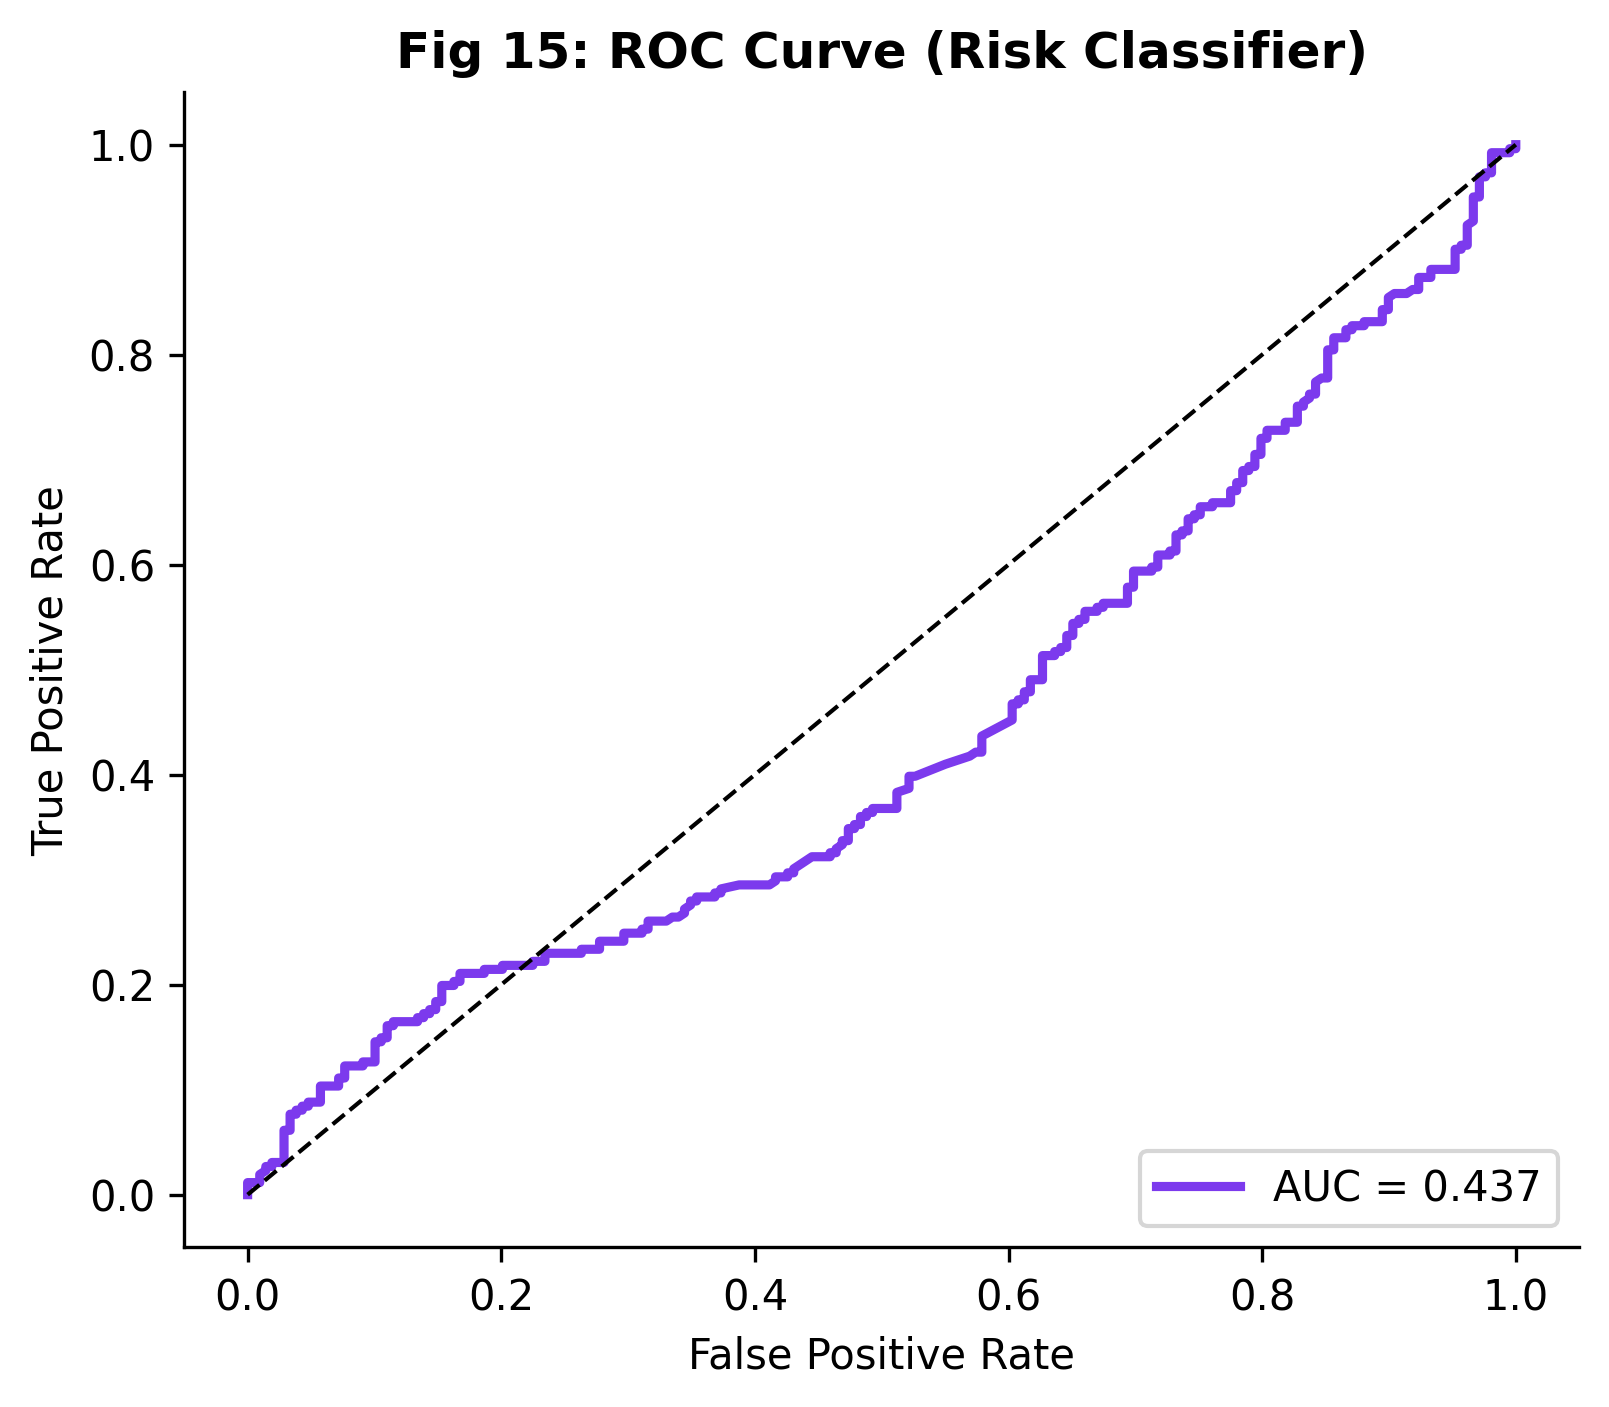
\includegraphics[width=0.85\columnwidth]{15_roc_curve.png}
\caption{ROC curve for the sigmoid-calibrated binary classifier. The AUC reflects the noise inherent in cross-dataset linkage, not a deficiency in the learning algorithm itself.}
\label{fig:roc}
\end{figure}

\subsection{Predictor Ranking}

Fig.~\ref{fig:feat} shows the ten model features ranked by impurity-based importance from the explanation proxy forest. Age sits at the top, trailed by Stress Level and Cycle Day. The three rolling-window features---Stress Volatility, Stress Rolling Mean, Sleep Rolling Mean---together account for a meaningful slice of total importance, which reinforces the intuition that even a simple 3-day average captures behavioral dynamics that point-in-time values alone cannot. This result, in retrospect, justified the design decision to invest engineering effort in rolling-window feature construction despite the limited overall discrimination power of the classifier.

\begin{figure}[t]
\centering
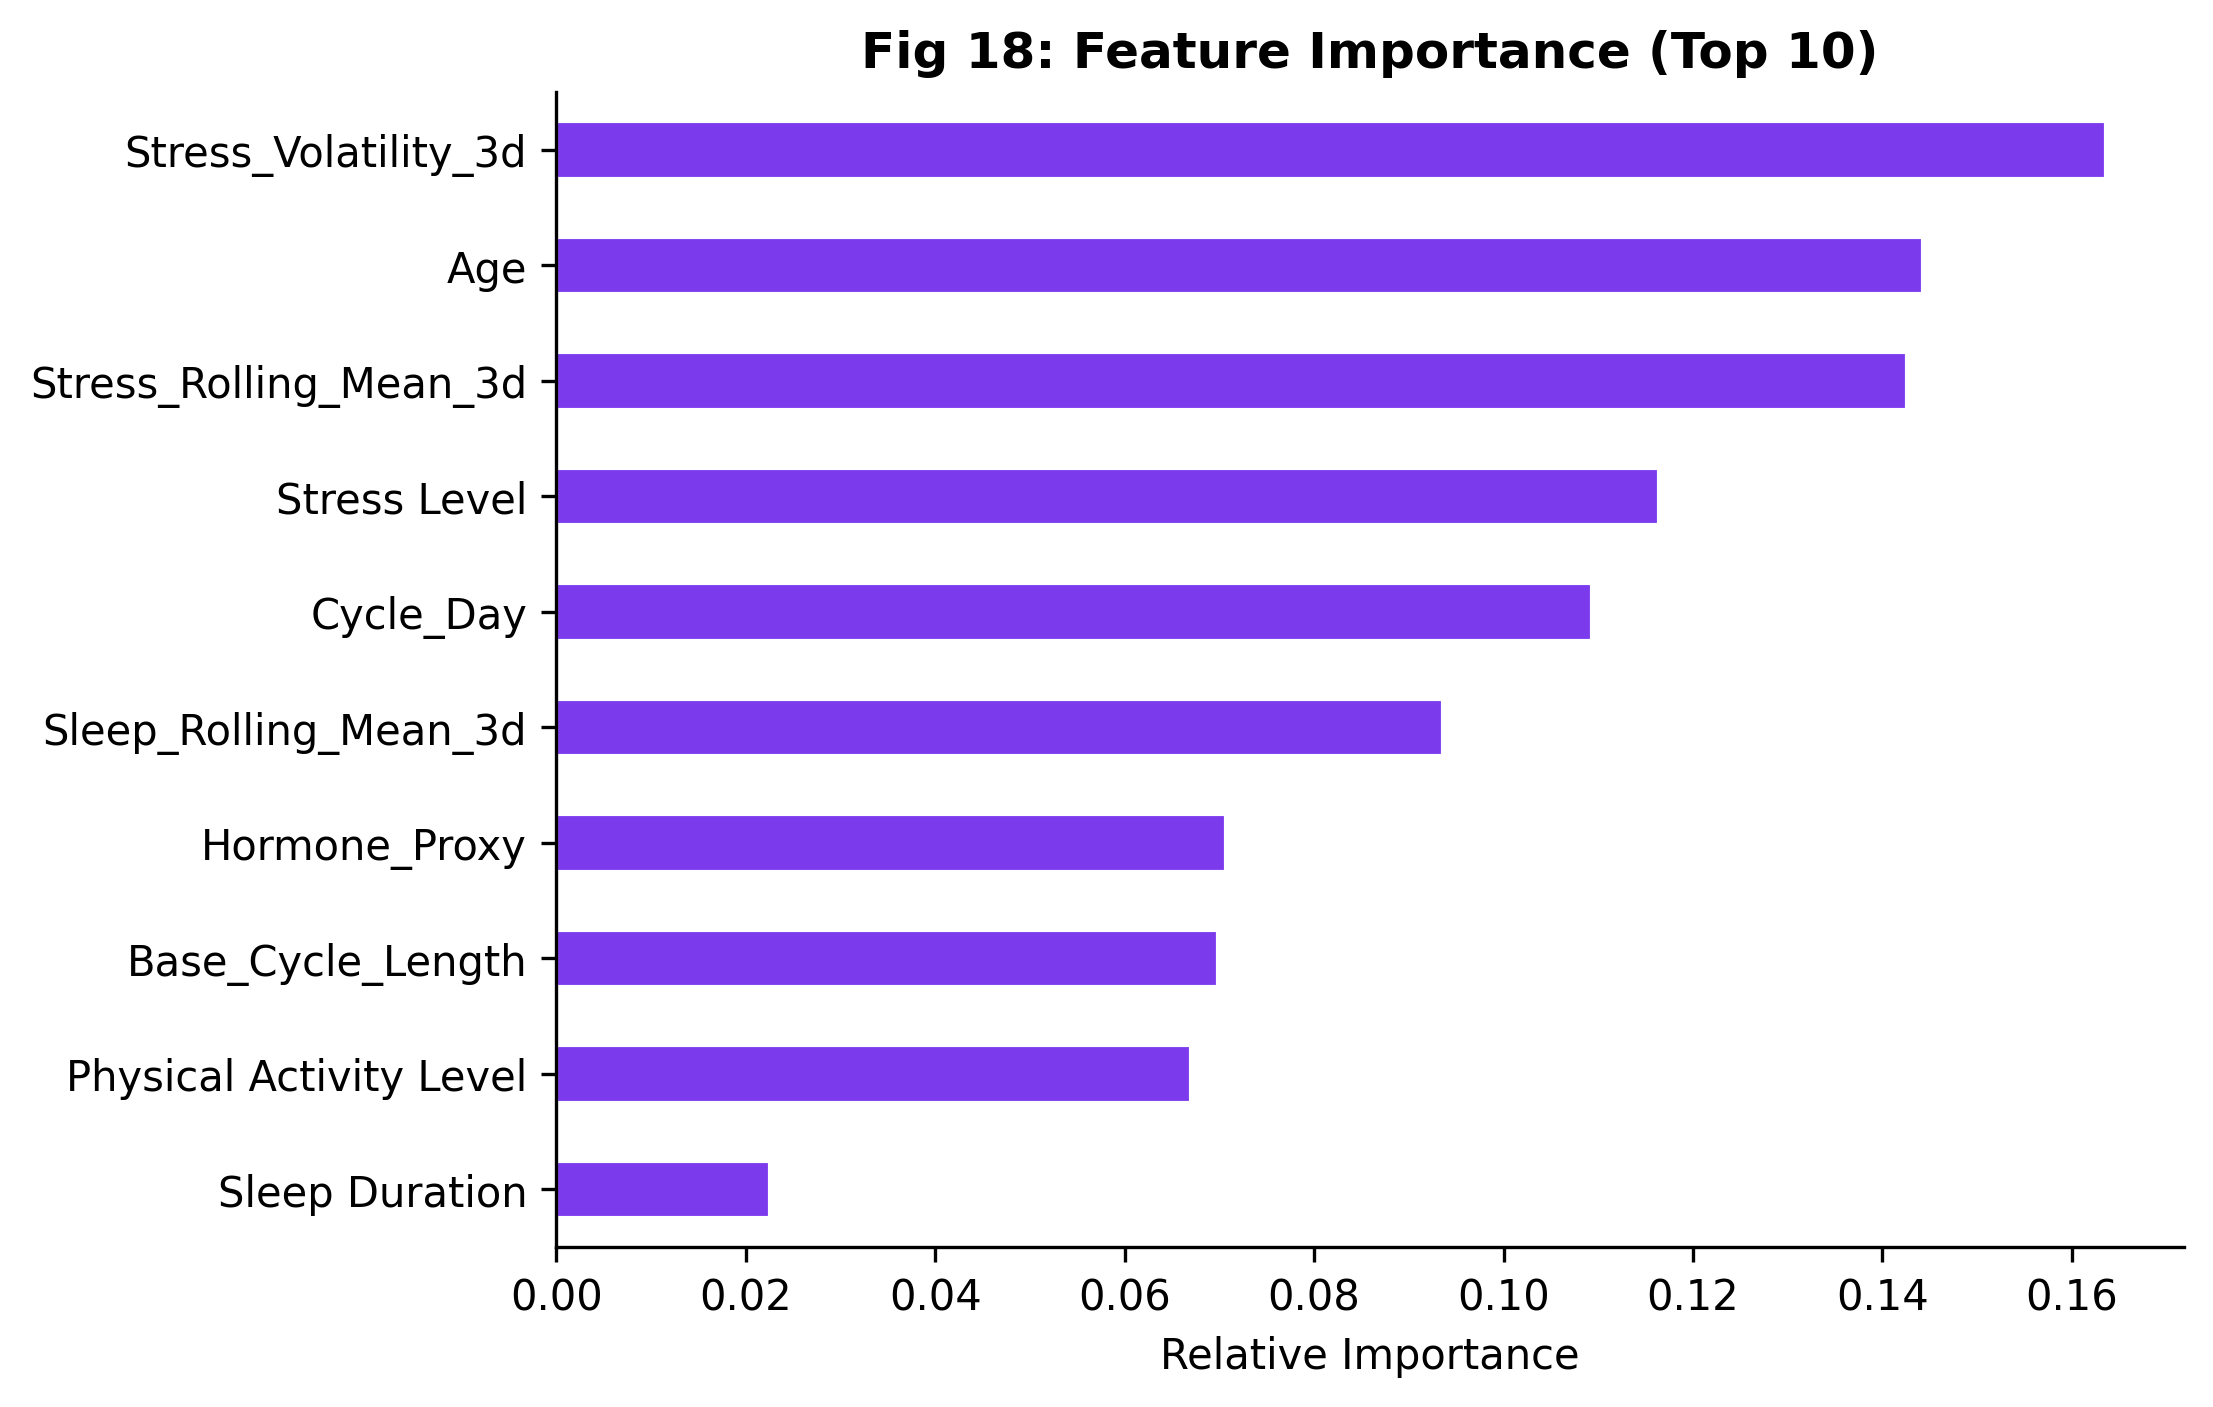
\includegraphics[width=0.85\columnwidth]{18_feature_importance.png}
\caption{Feature importance from the 100-tree explanation proxy. Temporal rolling features contribute non-trivially, supporting the inclusion of short-window longitudinal encoding.}
\label{fig:feat}
\end{figure}

\subsection{Formula Sensitivity}

Each input variable was swept across its full range with the remaining inputs fixed at baseline to confirm that the deterministic formula produces graded, directionally correct responses. Fig.~\ref{fig:sens} traces the stress dimension. Risk rises from roughly 15 at stress level 1 to around 55 at stress level 8; the Moderate threshold of 35 is crossed near stress 5.5. Reaching the High tier ($R \geq 65$) demands simultaneous adversity on more than one axis---elevated stress together with short sleep or high anxiety, for example. This multi-factor gating is intentional: it prevents any single extreme value from, by itself, pushing a user into the highest severity band. The observed transition points sit comfortably within ranges that the stress--health literature considers clinically plausible \cite{mcewen2008central}.

\begin{figure}[t]
\centering
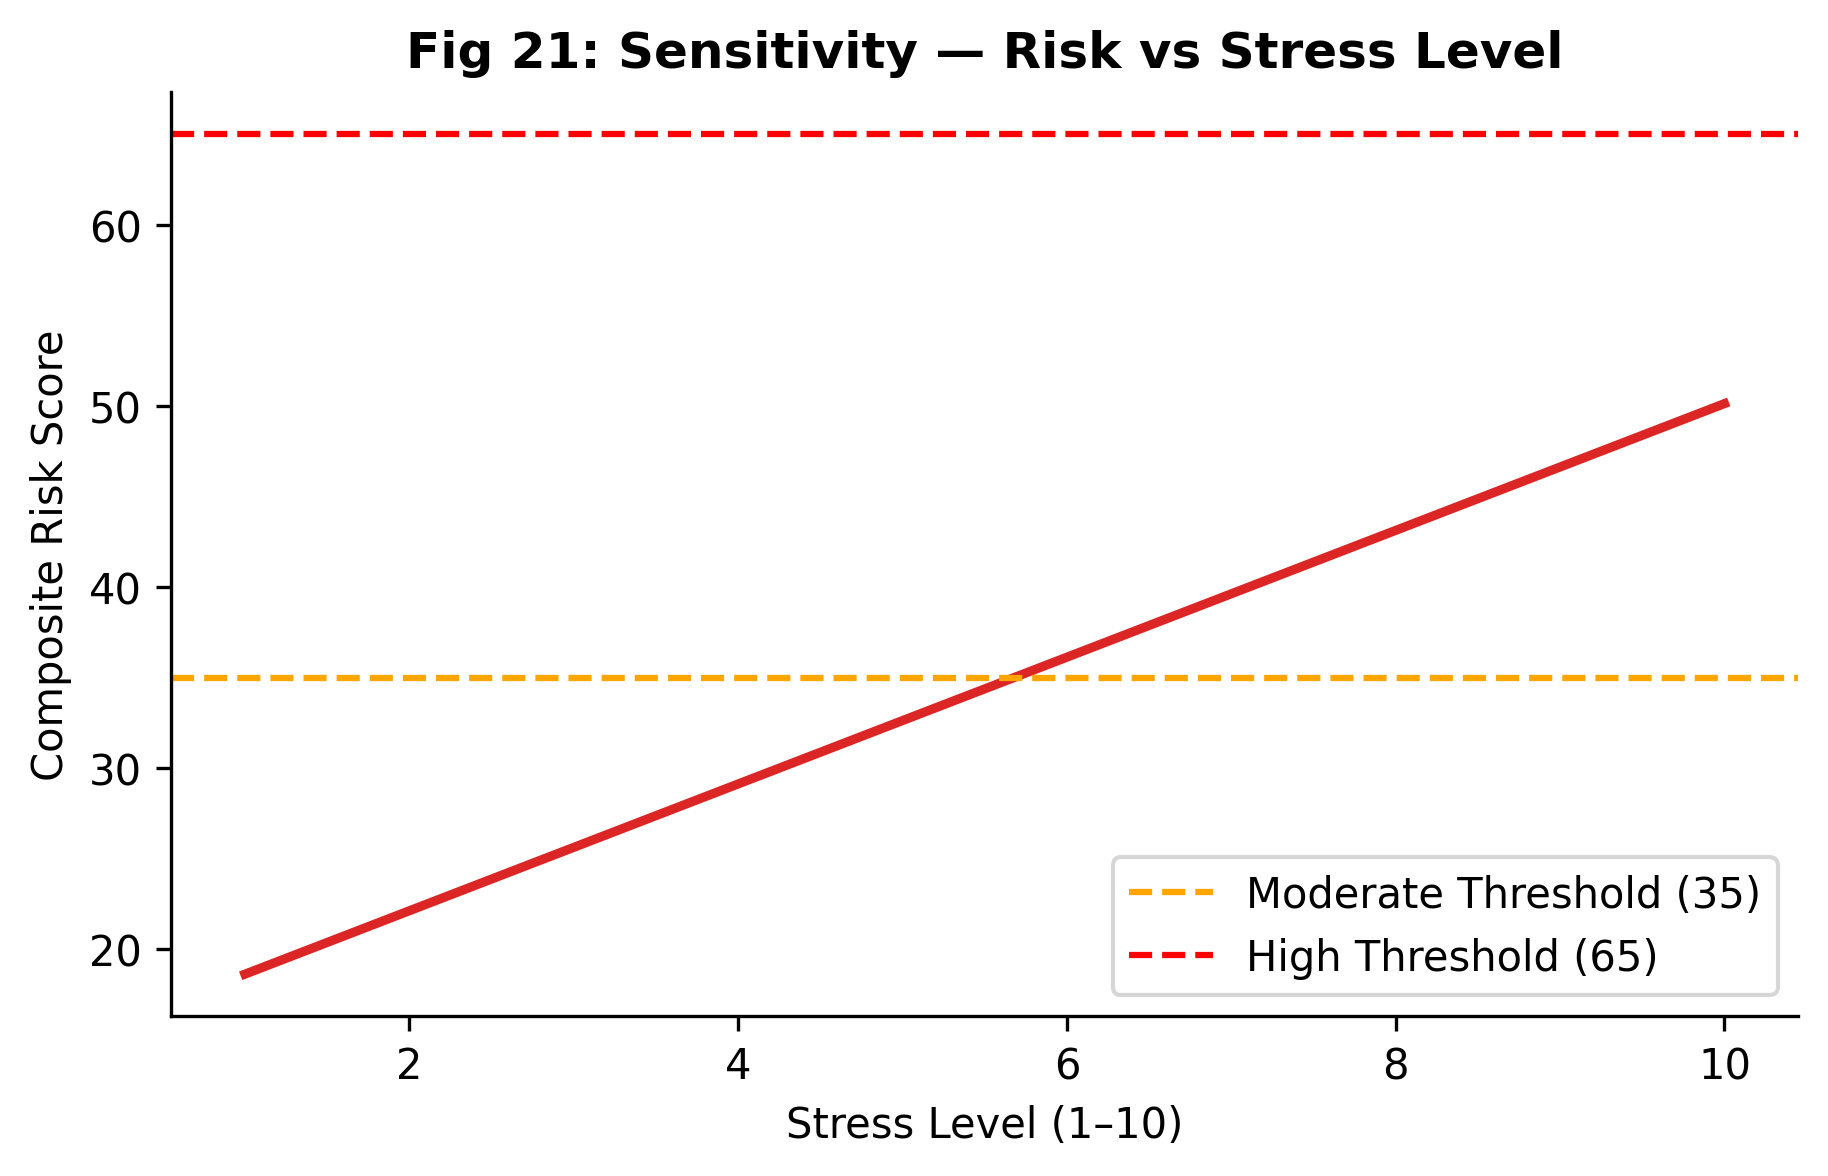
\includegraphics[width=0.85\columnwidth]{21_sensitivity_risk_vs_stress.png}
\caption{Risk score versus stress level (remaining inputs at baseline). Dashed lines indicate the Moderate (35) and High (65) tier boundaries.}
\label{fig:sens}
\end{figure}

\subsection{Hormonal Phase Effects}

Fig.~\ref{fig:cycle} holds all non-cycle inputs constant and varies only the menstrual phase. The Luteal window (days 17--28, $\phi = +8$) elevates baseline risk to roughly 36---nudging it just past the Moderate threshold---while the Ovulatory window (days 14--16, $\phi = -8$) pulls it down to about 20. Sixteen points of spread may look modest on a 100-point ruler, and that is by design. Hormonal context, in our conception, should adjust the overall picture without overwhelming it. The published effect sizes for cycle-related mood and sleep disruption are themselves moderate \cite{baker2007sleep, kiesner2012menstrual}, and we saw no reason to exaggerate them computationally.

When a user identifies as Male or selects Other, $\phi$ is set to zero. The 10\% of total capacity that would have served cycle context is rerouted to sleep deficit (25\% $\to$ 30\%), keeping the weight sum intact (Table~\ref{tab:weights}).

\begin{figure}[t]
\centering
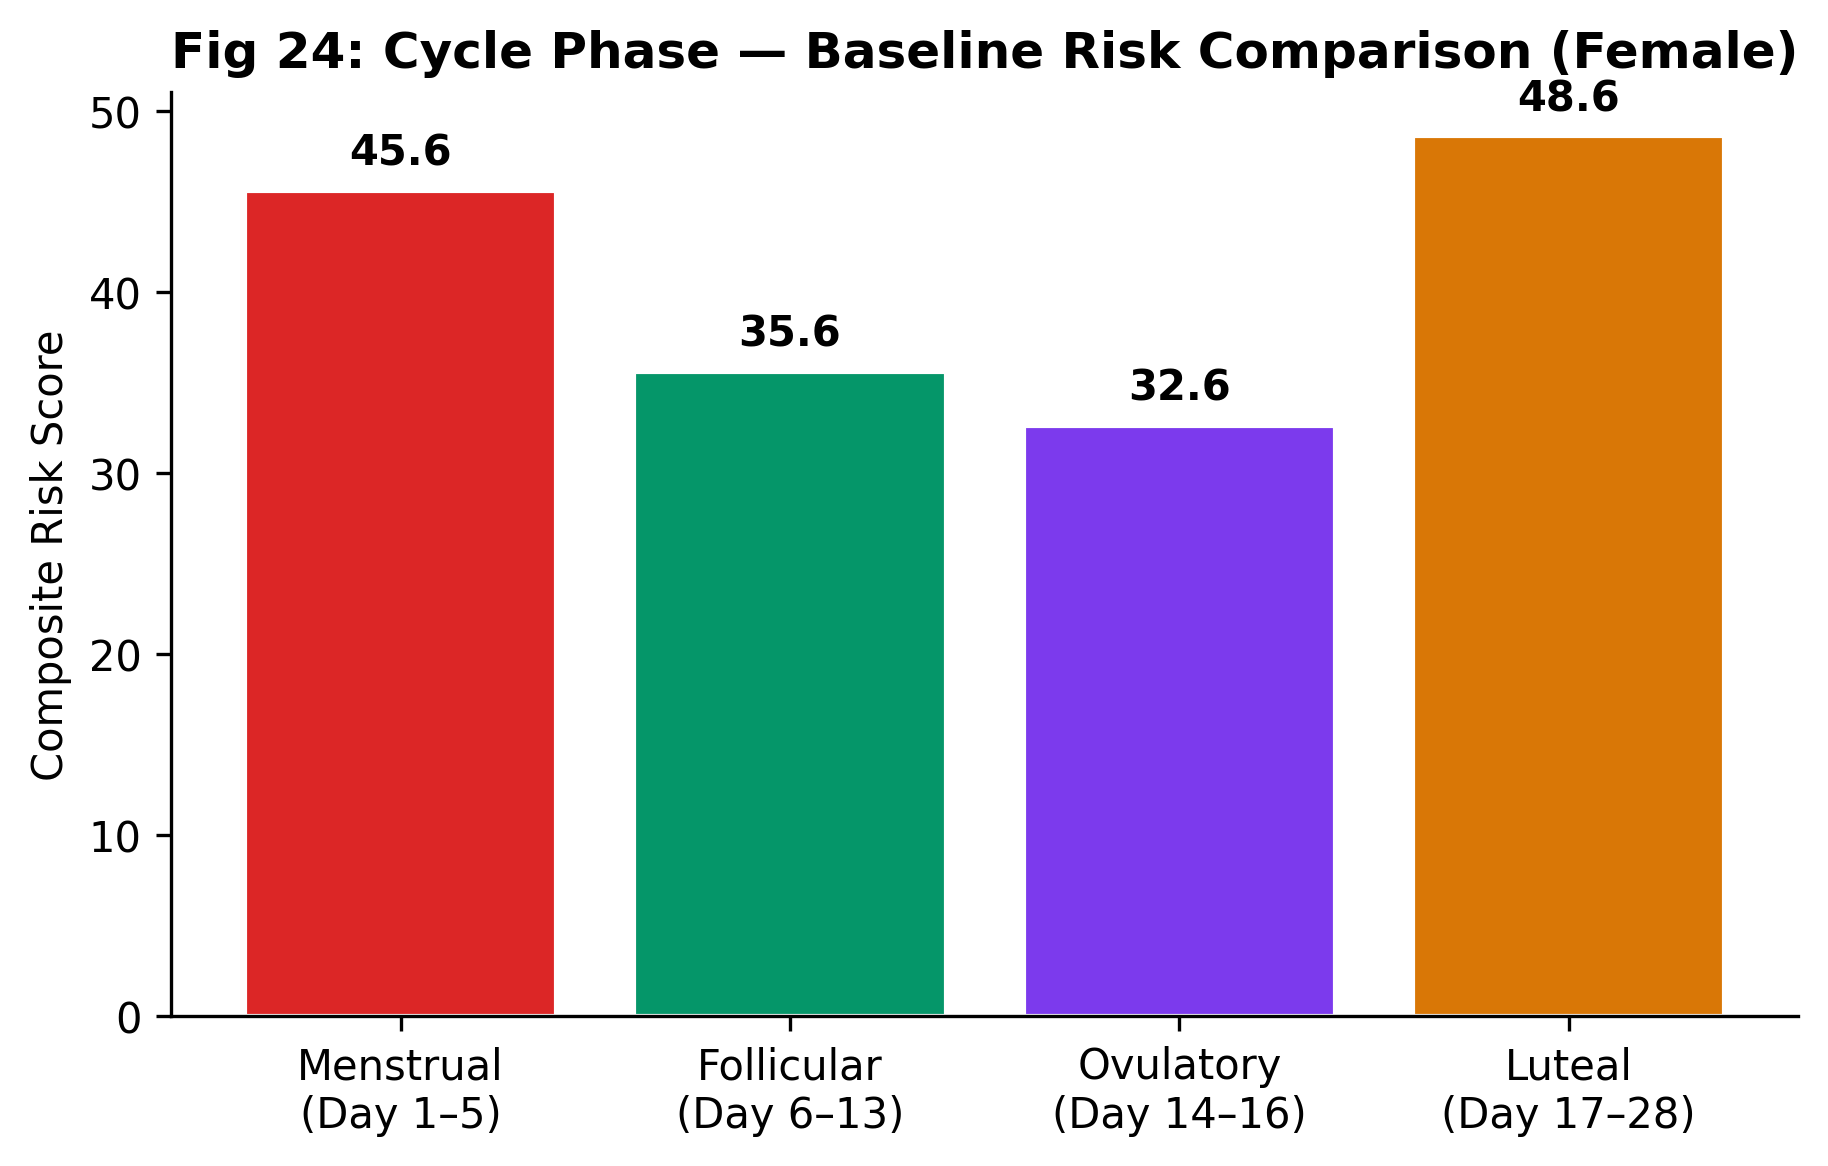
\includegraphics[width=0.85\columnwidth]{24_cycle_phase_comparison.png}
\caption{Baseline risk across menstrual phases (female profiles). Luteal and Menstrual windows raise risk; Follicular and Ovulatory windows lower it.}
\label{fig:cycle}
\end{figure}

\begin{table}[t]
\centering
\caption{Gender-Adaptive Weight Allocation in the Composite Risk Formula}
\label{tab:weights}
\begin{tabular}{lcc}
\toprule
\textbf{Factor} & \textbf{Female} & \textbf{Male / Other}\\
\midrule
Stress & 35\% & 35\%\\
Sleep Deficit & 25\% & 30\%\\
Anxiety & 20\% & 20\%\\
Activity Deficit & 10\% & 10\%\\
Hydration Deficit & 5\% & 5\%\\
Phase Modifier & $\pm$5--8 pts & 0\\
Trend Baseline & 5 pts & 5 pts\\
\bottomrule
\end{tabular}
\end{table}

\subsection{Justification for the Hybrid Design}

One might reasonably ask whether the ML components, given their limited standalone discrimination, add enough value to justify the added complexity. We believe they do, and for four separate reasons. The deterministic formula handles the primary score and keeps it auditable---users can see exactly how their inputs translate. The calibrated classifier contributes a probability shaped by the entire PHQ-9 feature space, picking up nonlinear interactions that a linear sum cannot represent. The quantile regressors generate confidence bands, something no static formula is capable of, which lets the dashboard convey how certain (or uncertain) any given estimate really is. And the SHAP proxy converts abstract model internals into plain-English attribution statements, powering the ``Personalized Insights'' panel that separates this dashboard from a bare numerical display.

\subsection{Limitations}

An honest accounting of constraints is warranted. The evaluation cohort is entirely synthetic. Although its feature ranges were chosen to span realistic territory, it cannot replicate the tangled interdependencies present in organically collected behavioral data. The formula weights are expert-informed heuristics, not the product of optimization against verified clinical endpoints. The classifier's modest AUROC is a direct artifact of cross-dataset linkage; it would almost certainly rise with a natively integrated training corpus. Cycle-phase modifiers represent population averages and make no attempt to personalize to an individual's unique hormonal response curve. And the point bears repeating one final time: every output this system produces is a Behavioral Wellness Estimate. It is not, and should not be read as, a clinical diagnosis.

%-----------------------------------------------------------------------
\section{Conclusion and Future Work}
%-----------------------------------------------------------------------

This paper described LunaAura, a framework that unites deterministic composite scoring, calibrated probabilistic classification, quantile-based uncertainty estimation, and instance-level SHAP attribution inside a longitudinal behavioral health dashboard. The central argument is straightforward: cycle-aware, gender-adaptive wellness analytics can be assembled from well-understood ML building blocks and transparent formulas, without falling back on opaque end-to-end architectures or overstated performance claims.

Several avenues for future work present themselves, organized here by priority. On the clinical front, the most pressing need is evaluation against longitudinal datasets gathered under institutional review, with psychiatrist-confirmed outcomes serving as ground truth. On the engineering side, coupling the platform with wearable device APIs---heart-rate variability, actigraphy, automated sleep staging---would shift the input balance from exclusively self-reported toward a mix of active and passive signals \cite{torous2021digital}. On the architectural side, a federated learning setup \cite{wu2021federated} would make it possible to refine models across geographically dispersed user groups without pooling raw behavioral records in a central repository, a property that any privacy-sensitive deployment will eventually require. Smaller planned improvements include Bayesian weight optimization conditioned on clinical outcomes, a native mobile client for daily use, and individualized cycle-length modeling to replace the current fixed 28-day assumption.

The complete source code, trained model files, database schemas, and evaluation scripts are hosted in the project repository and available for independent inspection, replication, and extension.

\bibliographystyle{IEEEtran}
\bibliography{references}

\end{document}
